\documentclass[11pt,oneside]{article}
\usepackage[T1]{fontenc}
\usepackage[utf8]{inputenc}
\usepackage[french]{babel}
\usepackage[autolanguage]{numprint} 
\usepackage{hyphenat}
\usepackage[breakable]{tcolorbox}
\usepackage[utf8]{inputenc}

\usepackage[a4paper,top=2cm,bottom=2cm,left=3cm,right=3cm,marginparwidth=1.75cm]{geometry}

\usepackage{amsmath, amsthm, amssymb, amsfonts}
\usepackage{graphicx}
\usepackage[colorlinks=true, allcolors=blue]{hyperref}

\usepackage[lined,linesnumbered]{algorithm2e}
\usepackage{url}
\usepackage[colorlinks=true, allcolors=blue]{hyperref}
\usepackage{graphicx} 
\usepackage{booktabs} 
\usepackage{amssymb}
\usepackage{minitoc}
\usepackage{enumitem}
\usepackage{tikz}               
\usetikzlibrary{calc}         
\usepackage{tkz-graph}

\usepackage{caption}
\usepackage{subcaption}
\usepackage{minitoc}


\usepackage{setspace}
\usepackage{geometry}
\usepackage{float}
\usepackage{hyperref}
\usepackage[utf8]{inputenc}
\usepackage[french]{babel}
\usepackage{framed}
\usepackage[dvipsnames]{xcolor}
\usepackage{tcolorbox}


\newtheorem{theorem}{Théorème}
\newtheorem{property}[theorem]{Propriété}
\newtheorem{properties}[theorem]{Propriétés}
\newtheorem{definition}[theorem]{Définition}
\newtheorem{notation}[theorem]{Notation}
\newtheorem{notations}[theorem]{Notations}
\newtheorem{admis}[theorem]{Hypothèse}

\newenvironment{ficheId}
{\begin{center}
    \begin{tabular}{p{0.9\textwidth}}
    \\
    \textbf{Fiche Identité:}
    }
    { 
    \\
    \end{tabular} 
    \end{center}
    }

\newenvironment{resume}
{\begin{center}
    \begin{tabular}{p{0.7\textwidth}}
    \\
    \textbf{Résumé:}
    }
    { 
    \\
    \end{tabular} 
    \end{center}
    }    



\usepackage[backend=biber,style=authoryear,natbib=true]{biblatex}
\addbibresource{bibliography.bib} % Link your .bib file here


\usepackage{graphicx} % Required for inserting images
\usepackage{geometry}
\usepackage{amssymb}
\usepackage{amsmath}
\geometry{hmargin=2.5cm,vmargin=1.5cm}
\usepackage[T1]{fontenc}
\usepackage[utf8]{inputenc}
\usepackage[french]{babel}
\usepackage[autolanguage]{numprint} 
\usepackage{hyphenat}
\usepackage[breakable]{tcolorbox}
\title{Per-chapter bibliographies with BibLaTeX}

\usepackage[a4paper,top=2cm,bottom=2cm,left=3cm,right=3cm,marginparwidth=1.75cm]{geometry}




\geometry{
    textheight=9in,
    textwidth=5.5in,
    top=1in,
    headheight=12pt,
    headsep=25pt,
    footskip=30pt
}


\usepackage{amsmath, amsthm, amssymb, amsfonts}
\usepackage{graphicx}
\usepackage[colorlinks=true, allcolors=blue]{hyperref}

\usepackage[lined,linesnumbered]{algorithm2e}
\usepackage{url}
\usepackage[colorlinks=true, allcolors=blue]{hyperref}
\usepackage{graphicx} 
\usepackage{booktabs} 
\usepackage{amssymb}
\usepackage{amsmath}
\usepackage{amssymb}
\usepackage{minitoc}
\usepackage{enumitem}
\usepackage{tikz}               
\usetikzlibrary{calc}         
\usepackage{tkz-graph}

\usepackage{caption}
\usepackage{subcaption}
\usepackage{minitoc}


\usepackage{setspace}
\usepackage{geometry}
\usepackage{float}
\usepackage{hyperref}
\usepackage[utf8]{inputenc}
\usepackage[french]{babel}
\usepackage{framed}
\usepackage[dvipsnames]{xcolor}
\usepackage{tcolorbox}



\title{Matrices circulantes et propriétés de la Transformée de Fourier Discrète}
\author{Hector Blondel}
\date{November 2024}





\begin{document}

\maketitle

\begin{ficheId}
\begin{center}
\begin{tabular}{|l|l|}
\hline
Discipline & Mathématiques \\
\hline
Auteur  & Hector Blondel \\
\hline
Année   & 2024-2025 \\
\hline
Cours concerné  & Traitement du signal \\
\hline
Relu par & \\
\hline
\end{tabular}
\end{center}
\end{ficheId}

\begin{resume}
La transformée de Fourier discrète se définit naturellement et hérite de propriétés similaires à celles de la transformée de Fourier classique. Elle peut-être vue comme une opération linéaire (et donc ayant sa matrice associée). Le formalisme matriciel permet de retrouver beaucoup de propriétés de la transformée de Fourier discrète, comme le théorème de convolution (la transformée de Fourier de la convolution circulaire de deux vecteurs est également le produit terme-à-terme des transformées de Fourier de ces deux vecteurs)  \\

\textbf{Mots-clés} : Traitement numérique du signal, Transformée de Fourier, convolution circulaire, matrice circulante
\end{resume}

\minitoc





\section*{Introduction}

Que ce soit pour l'analyse de signaux temporels, ou en télécommunications pour a transmission d'information ou , la transformation de Fourier est omniprésente dans la plupart des applications d'ingénieurie. Bien que notre monde soit physique et continu, l'ingénieur doit se résilier à manipuler informatiquement des signaux à durée fini et à temps discret. La transformée de Fourier discrète est alors nécessaire.

Nous nous proposons ici d'introduire la transformée de Fourier discrète, sous un angle matriciel, en compléménet du cours de première année de traitement du signal de Centrale-Supélec. Cet angle permettra au lecteur de visulaliser plus facilement ce qui se passe, et de pouvoir vérifier ou redémontrer facilement les propriétés.

\begin{notations}


Soit $N \in \mathbb{N}$. Nous notons $\mathcal{M}_n(\mathbb{C})$ l'ensemble des matrices carrées de taille $N$ à coefficients dans $\mathbb{C}$. Les coefficients des matrices seront indicés de $0$ à $N-1$ : 
$\forall (i,j) \in [\![0,N-1]\!]^2$, $[M]_{i,j}$ désigne le coefficient $i,j$ de $M \in \mathcal{M}_n(\mathbb{C})$ et $x_i$ désigne le coefficient $i$ du vecteur $x \in \mathbb{C}^N$.


\end{notations}


\section{Matrices circulantes}





% \begin{tcolorbox}[colback=yellow!10!white,colframe=black!75!black,title=Definition: matrices de Toeplitz]
%      L'application 
% $$\tau : \begin{cases}
% \mathbb{C}^(N \to \mathcal{M}_N(\mathbb{C})  \\
% x = (x_{-N+1} \ldots, x_0, \ldots, x_{N-1}) \mapsto 
% \begin{bmatrix} 
% x_0 & x_1 & \cdots & x_{N-1} \\ 
% x_{-1} & x_0 & \cdots & x_{N-2} \\ 
% \vdots & \vdots & \ddots & \vdots \\ 
% x_{-N+1} & x_{-N+2} & \cdots & x_0 \\ 
% \end{bmatrix}
% \end{cases}$$ est un morphisme de groupe de $(\mathbb{C}^N ; +)$ vers $(\mathcal{M}_N(\mathbb{C}), +)$

% Nous appelons "matrices de toeplitz" l'image de $\tau$. C'est un sous-espace vectoriel de \mathcal{M}_N(\mathbb{C})$$
% \end{tcolorbox}







\begin{tcolorbox}[colback=yellow!10!white,colframe=black!75!black,title=Definition: matrices circulantes]
     L'application 
$$C : \begin{cases}
\mathbb{C}^N \to \mathcal{M}_N(\mathbb{C})  \\
x = (x_0, \ldots, x_{N-1}) \mapsto 
\begin{bmatrix} 
x_0 & x_1 & \cdots & x_{N-1} \\ 
x_{N-1} & x_0 & \cdots & x_{N-2} \\ 
\vdots & \vdots & \ddots & \vdots \\ 
x_1 & x_2 & \cdots & x_0 \\ 
\end{bmatrix}
\end{cases}$$ est un morphisme de groupe de $(\mathbb{C}^N ; +)$ vers $(\mathcal{M}_N(\mathbb{C}), +)$

Nous appelons "matrices circulantes" l'image de C.


\end{tcolorbox}

Par la suite, nous noterons $\mathcal{C}$ l'ensemble des matrices circulantes.

Les matrices circulantes permettent de représenter algébriquement l'opération de convolution circulaire.

\begin{definition}{convolution circulaire}
    Soient $x,y \in \mathbb{C}^N$ deux vecteurs complexes.
    Le produit de convolution circulaire est le vecteur de $\mathbb{C}^N$ dont les coefficients sont :

    $$(x \circledast y)_m = \sum_{n=0}^{N-1} x_{m-n \mod N} y_{n} $$

    L'opérateur C défini plus haut nous permet d'exprimer facilement cette opération :

    $$x \circledast y = C(x)^T y$$
\end{definition}


\section{Transformée de Fourier discrète}

\subsection{Définition}

Nous rappelons ci-dessous la définition de la transformée de Fourier discrète.




\begin{tcolorbox}[colback=yellow!10!white,colframe=black!75!black,title=Definition: transformée de Fourier discrète]
    La transformée de Fourier discrète $\mathcal{F}(x)$ de $x = (x_0, x_1, ..., x_{N-1})$ est la suite de k éléments :
    $\mathcal{F}(x)_k = \tilde x_k = \sum_{n=0}^{N-1} x_n e^{-i\frac{2 \pi k n}{N}}$
\end{tcolorbox}

Posons $\omega = e^{- i \frac{2\pi}{N}}$.
Nous notons
$F = \frac{1}{\sqrt{N}}\begin{bmatrix}  
1 & 1 & 1 & \cdots & 1\\
1 & \omega & \omega^{2} & \cdots & \omega^{N-1}\\
\cdots & \cdots & \cdots & \cdots & \cdots\\
1 & \omega^{N-1} & \omega^{2(N-1)}& \cdots& \omega^{(N-1)(N-1)} 
\end{bmatrix}$ la matrice de Fourier. $[F]_{i,j} = \omega^{ij}$ : c'est la matrice de Van der Monde générée par les racines de l'unité d'ordre N.

La transformée de Fourier s'exprime simplement comme $\tilde x = \sqrt{N} F x$. Pour la suite, nous utiliserons les propriétés de la matrice $F$ pour démontrer les propriétés de la transformée de Fourier.

\begin{property}[proprietes de la matrice de Fourier]
\label{prop:matrice_Fourier}

\\

\begin{itemize}
    \item $F$ est unitaire : $F^H F = F F^H = I_N$
    \item $F$ est symmmétrique : $F^T = F$
\end{itemize}



\end{property}

\begin{proof}
    $\forall (i,j) \in [\![0,N-1]\!]^2,  [F^H F]_{l,m} = \sum_{k=0}^{N-1} [F^*]_{k,l} [F]_{k,m} = (\frac{1}{\sqrt{N}})^2 \sum_{k=0}^{N-1} e^{- i \frac{2 \pi k (l-m)}{N}} = \frac{1}{N} N \delta [l-m] = \delta [l-m] $
\end{proof}




Nous en déduisons directement l'expression de la transformée de Fourier discrète inverse : 
$$ \mathcal{F} = (\sqrt{N} F) \cdot \Rightarrow \mathcal{F}^{-1} = (\frac{1}{\sqrt{N}} {F^*}) \cdot $$ 
(nous avons aussi $\mathcal{F}^{-1} = \frac{1}{N} \mathcal{F}^*$)


\begin{tcolorbox}[colback=yellow!10!white,colframe=green!75!black,title=Propriétés de la Transformation de Fourier discrète]

Nous avons les propriété suivantes :

\begin{itemize}
    \item \textbf{Linéarité} : $\mathcal{F}\{a x + b y\} = a \tilde{x} + b \tilde{y}$, où $a$ et $b$ sont des scalaires complexes.
    \item \textbf{Symétrie hermitienne} : $x \in \mathbb{R} \Rightarrow \tilde{x}_{-k} = \tilde{x}_k^* \forall k \in [\![0,N-1]\!]$
    \item \textbf{Décalage dans le temps} :  $y_n = x_{n-m} \Rightarrow \mathcal{F}\{y\}_k = \mathcal{F}\{x\}_k e^{-j \frac{2\pi k m}{N}}, \forall k \in [\![0,N-1]\!]$.
    \item \textbf{Modulation} : Si  $y_n = e^{j \frac{2\pi n m}{N}} x_n \Rightarrow \mathcal{F}\{y\}_k = \mathcal{F}\{x\}_{k-m} \forall k \in [\![0,N-1]\!]$.

\end{itemize}

(Il est ici convenu que $\forall k \in \mathbb{N}$, $\mathcal{F}\{x\}_k := \mathcal{F}\{x\}_{k \mod N}$)

\end{tcolorbox}

    
\begin{property}
Toute matrice circulante $X \in \mathcal{C}$ est diagonalisable dans la base de Fourier (  $\begin{bmatrix}
1 \\
\omega^{k} \\
\omega^{2k}\\
... \\
\omega^{(N-1)k}
\end{bmatrix}$, $k \in [\![0,N-1]\!]$)

avec pour valeurs propres respectives les $\tilde x_k , k \in [\![0,N-1]\!]$ : 

$$X =  F \begin{bmatrix}
    \tilde x_0 &  &  &  \\
      & \tilde x_1 &   &  \\
     &  & \ddots &  \\
     &   &  & \tilde x_{N-1} \\
    \end{bmatrix} F^{-1} = F Diag(\tilde x)F^{-1}$$ 

\end{property}

\begin{proof}

soit $X = C(x_0, \cdots x_{N-1})$ une matrice circulante. Soit $k \in [\![0,N-1]\!]$. Nous avons  

\begin{align*}
[M \begin{bmatrix}
1 \\
\omega^{k} \\
\omega^{2k}\\
... \\
\omega^{(N-1)k}
\end{bmatrix}]_m = \sum_{n=0}^{N-1} x_{n-m \mod N} \omega^{nk}  \\
= \sum_{n=0}^{N-1} x_{n-m \mod N} \omega^{(n - m)k} \omega^{mk} 
= \sum_{n=0}^{N-1} x_{n-m \mod N} \omega^{(n - m \mod N)k}\omega^{mk}
\end{align*}. 

La dernière égalité vient du fait que  $\omega$ est une racine N-ième de l'unité.
$$\sum_{n=0}^{N-1} x_{n-m \mod N} \omega^{(n - m \mod N)k} \omega^{mk} =  (\sum_{n=0}^{N-1} x_{n} \omega^{nk}) \omega^{mk} = \tilde x_k \omega^{mk}$$.




Nous avons donc : 

$$
M \begin{bmatrix}
1 \\
\omega^{k} \\
\omega^{2k}\\
... \\
\omega^{(N-1)k}
\end{bmatrix} 
= \tilde x_k \begin{bmatrix}
1 \\
\omega^{k} \\
\omega^{2k}\\
... \\
\omega^{(N-1)k}
\end{bmatrix}
$$,
ce qui prouve bien que $\begin{bmatrix}
1 \\
\omega^{k} \\
\omega^{2k}\\
... \\
\omega^{(N-1)k}
\end{bmatrix} $ 
est vecteur propre pour la valeur propre $\tilde x_k$ de $M$. 

Puisque d'après \ref{prop:matrice_Fourier} ces $N$ vecteurs sont indépendants ($F$ est inversible), nous avons trouvé une base de vecteur propres et les matrices circulantes sont diagonalisables dans la base proposée. 


\end{proof}



Nous pouvons réécrire ce dernier résultat de manière matricielle : 

    
    
La précédente propriété nous permet de démontrer le théorème de convolution :


\begin{tcolorbox}[colback=yellow!10!white,colframe=purple!75!black,title=Théorème: Théorème de convolution]
    Soient $x$ et $y$ deux vecteurs de $\mathbb{C}^N$. Nous avons :
    $$\mathcal{F}\{x \circledast y \} = \mathcal{F} \{x\} \odot \mathcal{F} \{y\} $$ et 
    $$\mathcal{F}\{x \odot y \} = \frac{1}{N} (\mathcal{F} \{x\} \circledast \mathcal{F} \{y\}) $$, où $\odot$ désigne le produit de Hadamard (i.e. coefficient par coefficient) entre deux vecteurs. 
\end{tcolorbox}


\begin{proof}
    Nous avons : 
    $$x\circledast y = C(x)^T y = (F Diag(\tilde x) F^{-1})^T y = F^{-1} Diag(\tilde x) F y \Rightarrow \sqrt{N} F (x \circledast y) = Diag(\tilde x) \sqrt{N} F y$$. Cela nous donne donc bien, en identifiant terme à terme :
    
    $$\mathcal{F}\{x \circledast y \} = (\mathcal{F} \{x\}) \odot (\mathcal{F} \{y\}) $$
    En prenant $x = \mathcal{F}^{-1}\{x'\}$ et $y = \mathcal{F}^{-1}\{y'\}$ dans l'équation précédente : 
    \begin{align*}x' \odot y' = \mathcal{F}\{\mathcal{F}^{-1}\{x'\} \circledast \mathcal{F}^{-1}\{y'\} \}  =  \mathcal{F}\{\frac{1}{N}\mathcal{F}^*\{x'\} \circledast \frac{1}{N} \mathcal{F}^*\{y'\} \}
    \\
    \Rightarrow \frac{1}{N} \mathcal{F}^* \{x' \odot y'\}  = \mathcal{F}^{-1} \{x' \odot y'\} = \frac{1}{N}\mathcal{F}^*\{x'\} \circledast \frac{1}{N} \mathcal{F}^*\{y'\}  \end{align*}

    où la dernière ligne utilise que $\mathcal{F}^{-1} = \frac{1}{N} \mathcal{F}^*$.

    Finalement, nous obtenons le résultat attendu en prenant le conjugué et en multipliant par  $\frac{1}{N}$ des deux côtés de l'égalité.
    
    
\end{proof}


\subsection{Transformées de Fourier discrètes usuelles}


\begin{table}[H]
\centering
\begin{tabular}{|l|l|}
\hline
$\textbf{$x_n$}$ & $\tilde x_k = \mathcal{F}(x)_k$ \\ \hline
$x_n = \delta_{n_0}[n] $ & $\tilde x_k = e^{i\frac{2\pi n_0 n}{N}}$ \\ \hline
$x_n = e^{i \frac{2 \pi k_0 n}{N}}$ & $\tilde x_k = \delta_{k_0}[k] $ \\ \hline
$\frac{1}{n_0} 1_{[\![0,n_0 - 1]\!]}[n]$ & $e^{-i \pi \frac{k (n_0-1)}{N}} \frac{\sin{\frac{\pi k n_0}{N}}}{n_0 \sin{\pi \frac{k}{N}}}$  \\ \hline
\end{tabular}
\caption{Transformées de Fourier discrètes usuelles}
\label{tab:2cols}
\end{table}


Cette dernière fonction est l'équivalent discret du sinus cardinal continu. Nous avons tracé une représentation graphique ci-dessous : 


\begin{figure}[H]
    \centering
    % Première sous-figure
    \begin{subfigure}[b]{0.45\textwidth}
        \centering
        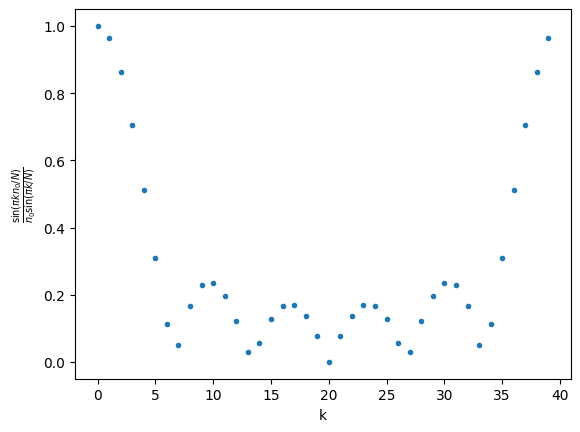
\includegraphics[width=\textwidth]{sinus_cardinal_decentre.png} % Remplacez par le chemin de votre image
        \caption{$k \in [\![0, N-1]\!]$}
        \label{fig:subfigure1}
    \end{subfigure}
    \hfill
    % Deuxième sous-figure
    \begin{subfigure}[b]{0.45\textwidth}
        \centering
        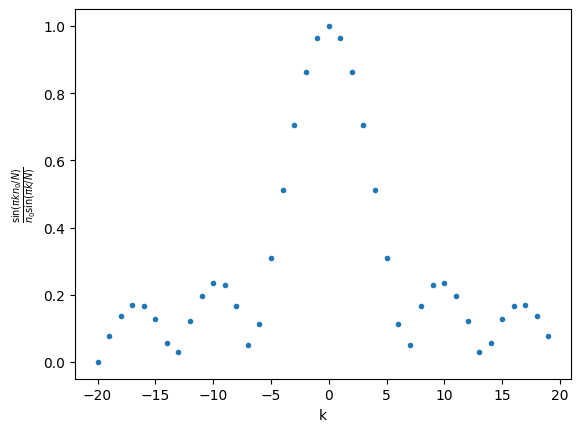
\includegraphics[width=\textwidth]{sinus_cardinal_centre.png} % Remplacez par le chemin de votre image
        \caption{$k \in [\![-\frac{N}{2}, \frac{N}{2} - 1]\!]$}
        \label{fig:subfigure2}
    \end{subfigure}
    % Légende globale
    \caption{tracé de $k \mapsto \frac{\sin(\frac{\pi k n_0}{N})}{n_0 \sin(\frac{\pi k}{N})}$}
    \label{fig:mainfigure}
\end{figure}

Il est plus naturel de représenter le sinus cardinal négatif sur $[\![-\frac{N}{2},\frac{N}{2} - 1]\!]$. Par périodicité, il s'agit d'une rotation cyclique des valeurs sur $[\![0,N-1]\!]$.

\underline{Exercice :}
Montrer que la transformée de Fourier discrète de la suite finie $( \begin{pmatrix}
N-1 \\
n
\end{pmatrix})_n$ est $((1+e^{i\frac{2 \pi k}{N}})^{N-1})_k$

\section{Implémentation algorithmique et applications}


\subsection{Implémentation : Fast Fourier Transform, transformée de Fourier rapide}


Le calcul naïf de la transformée de Fourier discrète recquiert de l'ordre de $N^2$ opérations (multiplications ou additions complexes) : pour chaque indice de fréquence $k$, il faut calculer la somme des $N$ composantes $(x_n e^{-i\frac{2\pi kn}{N}})_n$.

L'idée principale de la FFT repose sur une décomposition récursive du calcul de la DFT. En divisant le signal d'entrée en sous-séquences de tailles plus petites, on peut réduire le nombre d'opérations nécessaires.

Pour simplifier, supposons que $N$ est une puissance de 2. On peut écrire $x_n$ comme la somme de deux séquences :
\[
x_n = x_{\text{pair}}(n) + x_{\text{impair}}(n)
\]
avec :
\[
x_{\text{pair}}(m) = x_{2m}, \quad x_{\text{impair}}(m) = x_{2m+1}.
\]

La DFT peut alors être exprimée comme :
\begin{align*}
\tilde x_k = \sum_{m=0}^{N/2-1} x_{2m} e^{-i \frac{2\pi}{N} k(2m)} + \sum_{m=0}^{N/2-1} x_{2m+1} e^{-i \frac{2\pi}{N} k(2m+1)}.
\\ = \sum_{m=0}^{N/2-1} x_{2m} e^{-i \frac{2\pi}{N/2} km} + e^{-i \frac{2\pi}{N} k} \sum_{m=0}^{N/2-1} x_{2m+1} e^{-i \frac{2\pi}{N/2} km}.
\end{align*}


Pour $k \in $

En factorisant, cela donne :

Pour $k \in [\![0,N/2-1]\!]$,

$$\begin{cases} \tilde x_k =  \sum_{m=0}^{N/2-1} x_{2m} e^{-i \frac{2\pi}{N/2} km} + e^{-i \frac{2\pi}{N} k} \sum_{m=0}^{N/2-1} x_{2m+1} e^{-i \frac{2\pi}{N/2} km}.  \\
\tilde x_{\frac{N}{2} + k} = \sum_{m=0}^{N/2-1} x_{2m} e^{-i \frac{2\pi}{N/2} km} + e^{-i \pi} e^{-i \frac{2\pi}{N} k} \sum_{m=0}^{N/2-1} x_{2m+1} e^{-i \frac{2\pi}{N/2} km}
\end{cases}$$



$$ \Rightarrow \begin{cases} \tilde x_k =  \tilde x_k^{\text{pair}} + e^{-i \frac{2\pi}{N} k} \tilde x_k^{\text{impair}}  \\
\tilde x_{\frac{N}{2} + k} = \tilde x_k^{\text{pair}} - e^{-i \frac{2\pi}{N} k} \tilde x_k^{\text{impair}}
\end{cases}$$

où $\tilde x_k^{\text{pair}}$ et $\tilde x_k^{\text{impair}}$ sont les TFDs des sous-séquences de taille $N/2$.

Le processus se poursuit en décomposant chaque sous-séquence jusqu'à obtenir des séquences de taille 1, pour lesquelles la TFD est la valeur du coefficient. Si nous notons $T(N)$ la complexité du calcul de la TFD sur une liste de taille $N$ par l'algorithme de Cooley-Tuckey, nous avons :

$$\begin{cases}
    T(N) = 2T(\frac{N}{2}) + N \\
    T(1) = 0
\end{cases}$$

Le premier terme correspond au calcul des DFT des deux sous-séquences. Le deuxième terme de la somme correspond au calcul des $\tilde x_k$ en fonction de ces dernières valeurs.

En posant $p = \log_2 N$ et $S(p) = T(N=2^p)$, l'équation de complexité devient :

$$
\begin{cases}
S(p) = 2 S(p-1) + 2^p \\
S(0) = 0
\end{cases}
$$

Une récurrence immédiate donne : 

$$S(p) = p 2^p \Rightarrow T(N) = S(\log_2 N) =  N \log_2 N$$.

Cela est meilleur que la complexité naïve (de $N^2$).


%\subsection{Une autre optimisation : pruned FFT}

\subsection{Application : produit de convolution rapide}

Soient $x \in \mathbb{C}^p$ et $y \in \mathbb{C}^q$ deux vecteurs. Nous souhaitons calculer la convolution (discrète) $$x \ast y = (\sum_{k=0}^{p-1} x_k y_{m-k})_{0 \leq m < p + q}$$ (où $x_k = 0$ lorsque $k \notin [\![0,p-1]\!]$ et $y_k = 0$ lorsque $k \notin [\![0,q-1]\!]$ .

Le calcul naïf nécessite de l'ordre de $\mathcal{O}(pq)$ opérations élémentaires.

Le théorème deconvolution nous permet de réduire facilement la complexité cu calcul de $x \ast y$ : remarquons qu'un produit de convolution classique est une convolution circulaire si l'on étend suffisemment le support des vecteurs. 

Posons $N=p+q-1$ et notons respectivement $x^{(N)}$ et $y^{(N)}$ les vecteurs étendus de $x$ et $y$ avec $N$ éléments (avec $x^{(N)} = \begin{bmatrix}
    x ~ 0 \cdots 0
\end{bmatrix}$
et 
$y^{(N)} = \begin{bmatrix}
    y ~  0 \cdots 0
\end{bmatrix}$). 
$$x \ast y = x^{(N)} \circledast y^{(N)} = \mathcal{F}^{-1}\{\mathcal{F}(x^{(N)}\} \odot \mathcal{F}\{y^{(N)})\}$$

Cette méthodes nécessite les opérations suivantes: 
\begin{itemize}
    \item Calcul des deux transformées de Fourier ($\mathcal{O}(N \log_2 (N)$))
    \item Produit de Hadamard ($\mathcal{O}(N)$)
    \item Transformée de Fourier inverse ($\mathcal{O}(N \log_2 N)$)
\end{itemize}

La complexité de cette nouvelle méthode est en $\mathcal{O}((p+q) \log_2 (p+q) ) \ll \mathcal{O}(pq)$, elle accélère significativement le calcul de la convolution.

En python, la fonction \texttt{scipy.signal.convolve} du package \texttt{scipy} utilise l'astuce que nous venons d'exposer pour calculer de la convolution entre deux tableaux.

Les calculs de produits polynômes relevant également du calcul de convolution, ou les produits d'entiers peuvent également grandement être améliorés avec cette méthode.



\section{Memo}


\begin{tcolorbox}[title=Mémo, colframe=cyan!75!black, colback=yellow!5!white, coltitle=black]
\begin{itemize}
    \item \textbf{Définition :} 
    $$\mathcal{F}(x)_k = \tilde x_k = \sum_{n=0}^{N-1} x_n e^{-i\frac{2 \pi k n}{N}}$$
    $$\mathcal{F}^{-1}(\tilde x)_n = x_n = \sum_{k=0}^{N-1} x_k e^{i\frac{2 \pi n k}{N}}$$
    \item \textbf{Linéarité :} 
    $$\mathcal{F}\{a x + b y\} = a \tilde{x} + b \tilde{y}$$ 
    où $a, b \in \mathbb{C}$.
    \item \textbf{Symétrie hermitienne :} 
    $$x \in \mathbb{R} \Rightarrow \tilde{x}_{-k} = \tilde{x}_k^* \quad \forall k \in [\![0,N-1]\!]$$
    \item \textbf{Décalage dans le temps :} 
    $$y_n = x_{n-m} \Rightarrow \mathcal{F}\{y\}_k = \mathcal{F}\{x\}_k e^{-j \frac{2\pi k m}{N}}$$
    \item \textbf{Modulation :} 
    $$y_n = e^{j \frac{2\pi n m}{N}} x_n \Rightarrow \mathcal{F}\{y\}_k = \mathcal{F}\{x\}_{k-m}$$
     \item \textbf{Convolution :} 
    $$\mathcal{F}\{x \circledast y \} = \mathcal{F} \{x\} \odot \mathcal{F} \{y\}$$
    $$\mathcal{F}\{x \odot y \} = \frac{1}{N} \mathcal{F} \{x\} \circledast \mathcal{F} \{y\}$$
    
\end{itemize}
\end{tcolorbox}



\nocite{*} % Includes all entries from the bibliography file
\printbibliography


\end{document}



\subsection{Applications}

\subsubsection{Calcul de convolution}

L'algorithme de FFT est une valeur sûre, et permet parfois de simplifier des calculs de manière très astucieuse.
Un cas emblématique est le calcul de convolution discrète. Supposons que l'on doive calculer le produit de convolution entre deux liste finies $a = (a_0, \cdot , a_{p-1})$ et $b= (b_0, \cdot , b_{q-1}$,avec $p,q \in \mathbb{N}$. Ce calcul est équivalent à la multiplication de deux polynômes $A(X)=\sum_{n=0}^{p}a_nX^n$ et $B(X)=\sum_{n=0}^{p}b_nX^n$.


\begin{algorithm}
    
\end{algorithm}


Algorithme naïf : 



\end{document}
